\chapter{PNb data analysis}
\label{chapter:analysis_pNb}
Complementary to data from pp experiment data collected during pNb experiment was analyzed to find a $\Ls$ signal. Main scope of the studies was the same, although differences in collided system has forced some minor changes in analysis methods. As a result inclusive \css for $\Ls$ together with the reference state $\Lz \Kz$ were measured and compared to the previous HADES studies \cite{hades_Sz_pNb,hades_Lp_femtoscopy_pNb,hades_arnold_pNb,hades_Ksi_pNb}. It allows to broaden a knowledge about hyperons of a pNb reactions and to point key differences between proton-proton and proton-nucleon reactions.

\section{Data from pNb experiment}
The p(3.5 GeV)+Nb experiment was conducted in October 2008. The beam with kinetic energy 3.5 GeV was delivered by the SIS 18 synchrotron and aimed into a segmented, 12-fold target. Each target element had a diameter equal 1.25 mm and 0.45 mm of a thickness. The target parameters were adjusted to get a 2.8\% interaction probability. The trigger system was the same as for pp@3.5 GeV experiment with LVL1 trigger based on hits multiplicity in META detector and LVL2 trigger dedicated for di-lepton studies. During experiment an avrege beam intensity was $2 \times 10^6$ particles/s, what gave in total $3.2 \times 10^9$ LVL1 events recorded on tapes.  

\begin{figure}[ht]
  \centering
  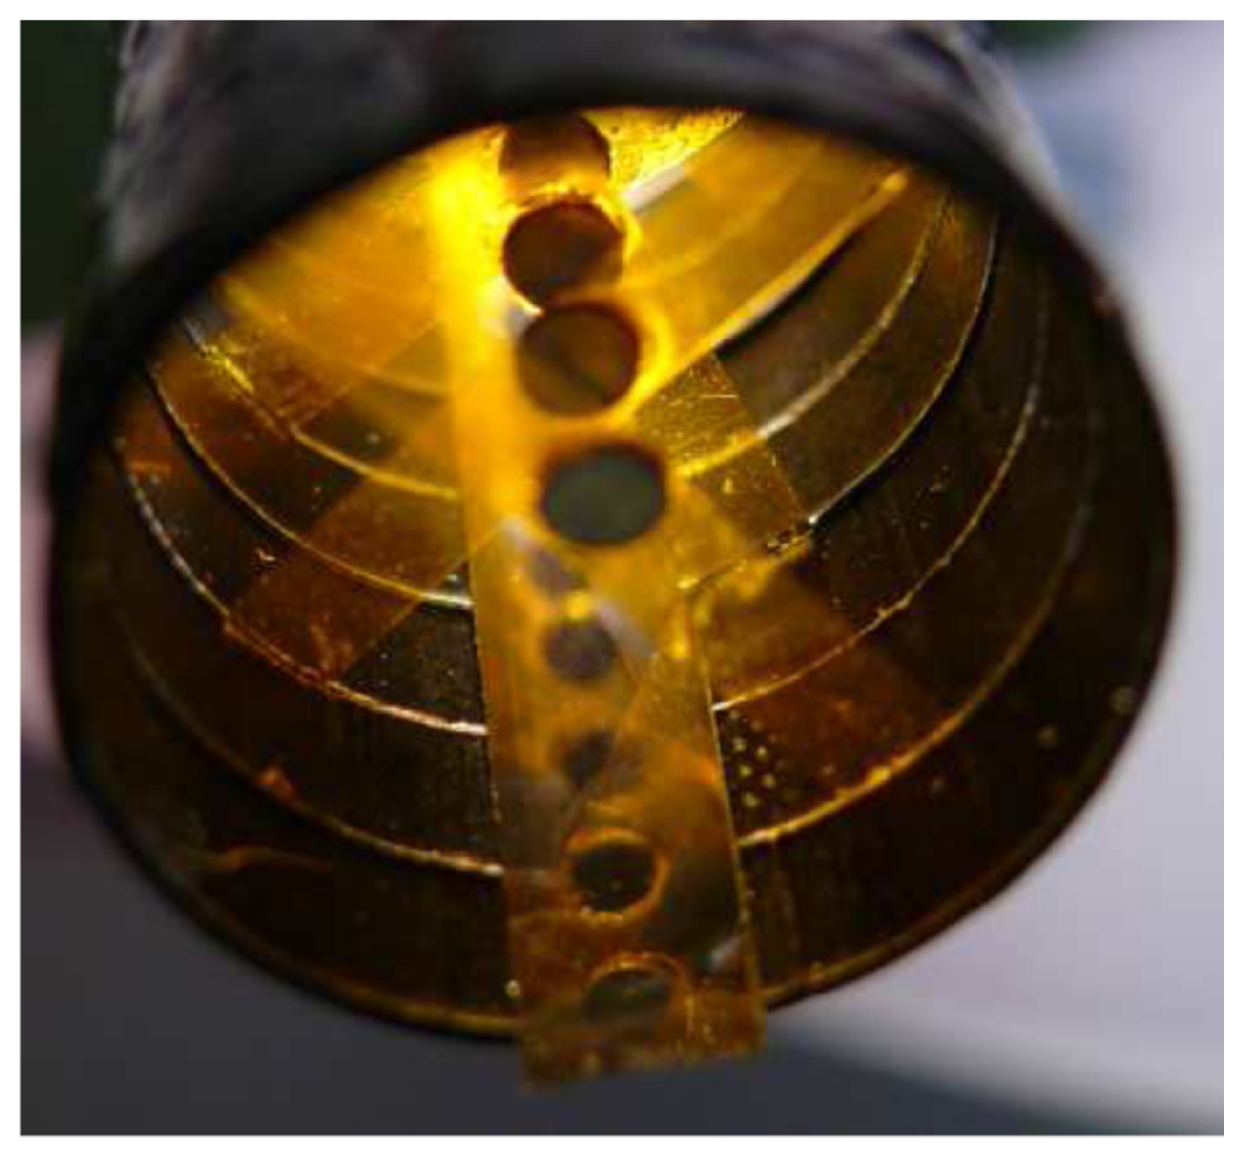
\includegraphics[width=0.7 \linewidth]{Chapter_analysisPNb/target_pNb.eps}
  \caption{The segmented niobium target used for an experiment. Niobium roundels are mounted by a tape inside a carbon tube.}
\end{figure}

\section{Identification and data selection}
Identification and selection algorithms used for pNb data were the same as in case of a pp data analysis. However in proton-nucleus reaction it is impossible to directly use the energy-momentum conservation rule. They are two main obstacles: part of four-momentum may be transferred to the nucleus as a recoil and nucleons in nucleus are not in rest. All together prevents from a use of the missing mass cut. The missing mass spectrum, in contrary to pp data, does not have any resonance behaviour. As a replacement a set of more restricted hard cuts was applied for  $\Lz$ reconstruction before a reconstruction done by the neural network.
\begin{figure}
  \centering
  \caption{The missing mass spectrum for $\p \pim \pip \pim$ hypothesis.}
  \label{fig:miss_mass_pNb}
\end{figure}

\section{The $\Lz$ Reconstruction}
The main tool for $\Lz$ reconstruction stays the same as for in chapter \ref{chapter:analysis}. It is a neural network trained in a data-driven manner. Although because of no missing mass cut obtained signal-to-background ratio was much lower than for pp case and it was.  The result is shown in fig. \ref{fig:L1116SB_pNb}.
\begin{figure}[ht]
  \centering
  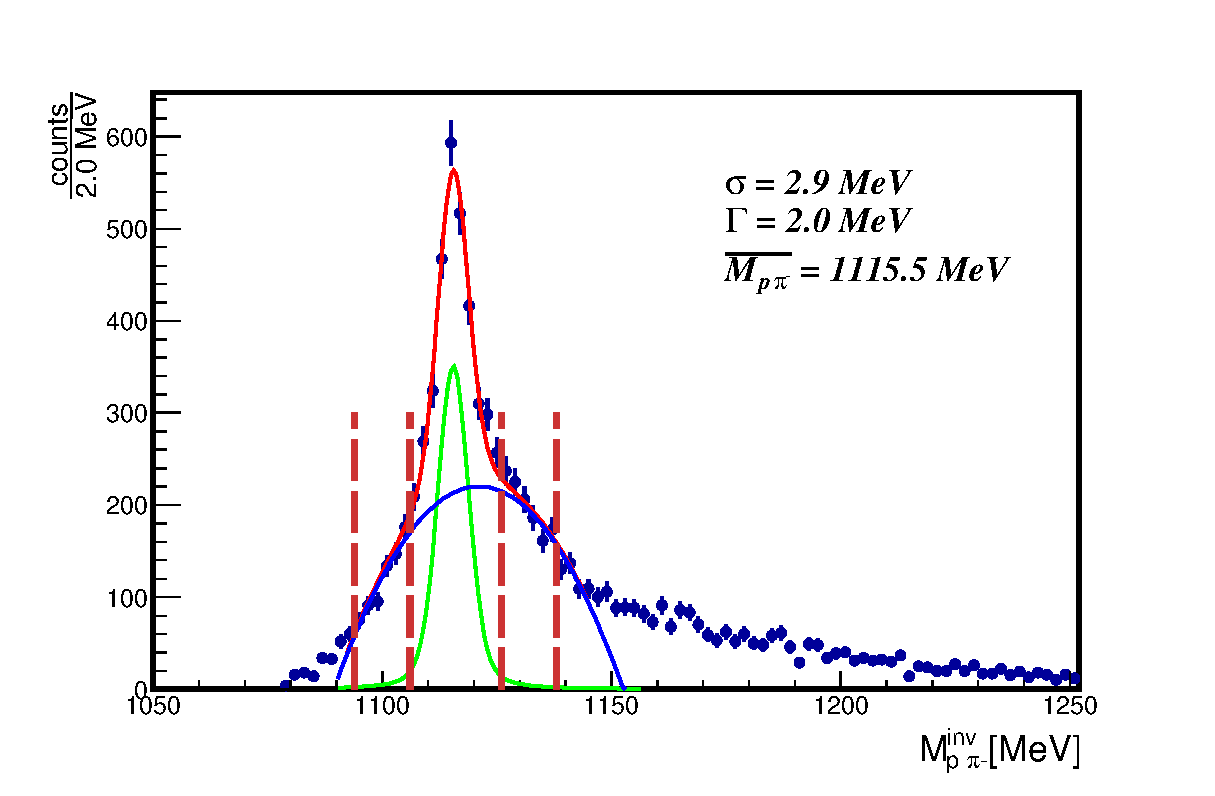
\includegraphics[width=0.7 \linewidth]{Chapter_analysisPNb/Lz.eps}
  \caption{The $\Lz$ spectrum after a neural network analysis obtained for pNb experiment. Color coding the same as in fig. \ref{fig:L1116SB}, vertical lines denotes regions of a side-band and were adjusted for pNb exclusively.}
  \label{fig:L1116SB_pNb}
\end{figure}

\section{The $\Lz \Kz $reconstruction}
The same as for in case of pp data an inclusive $\Lz \Kz$ production was a cross-check for en event selection method and absolute normalization. The normalization method used for a \cs extraction was the same like described in \ref{sec:normalization} with two quantitative differences. The first: a total luminosity for pNb experiment was ???, the second: a knowledge about inclusive \css for proton-nucleus scattering is strongly limited. Instead of exact values the universal scaling between reaction was assumed:
\begin{equation}
  \sigma_{pN}=\sigma_{pp} \cdot A^{2/3},
\end{equation}
where A is an atomic number of mass number of a given nucleus. The sam like in pp anaysis inclusive $\Lz$ production was estimated as a sum of explusife channels listed in tab. \ref{tab:channels}. The obtained simulation results gives well description for signals extracted from experimental data-set. 

\begin{figure}[ht]
  \centering
  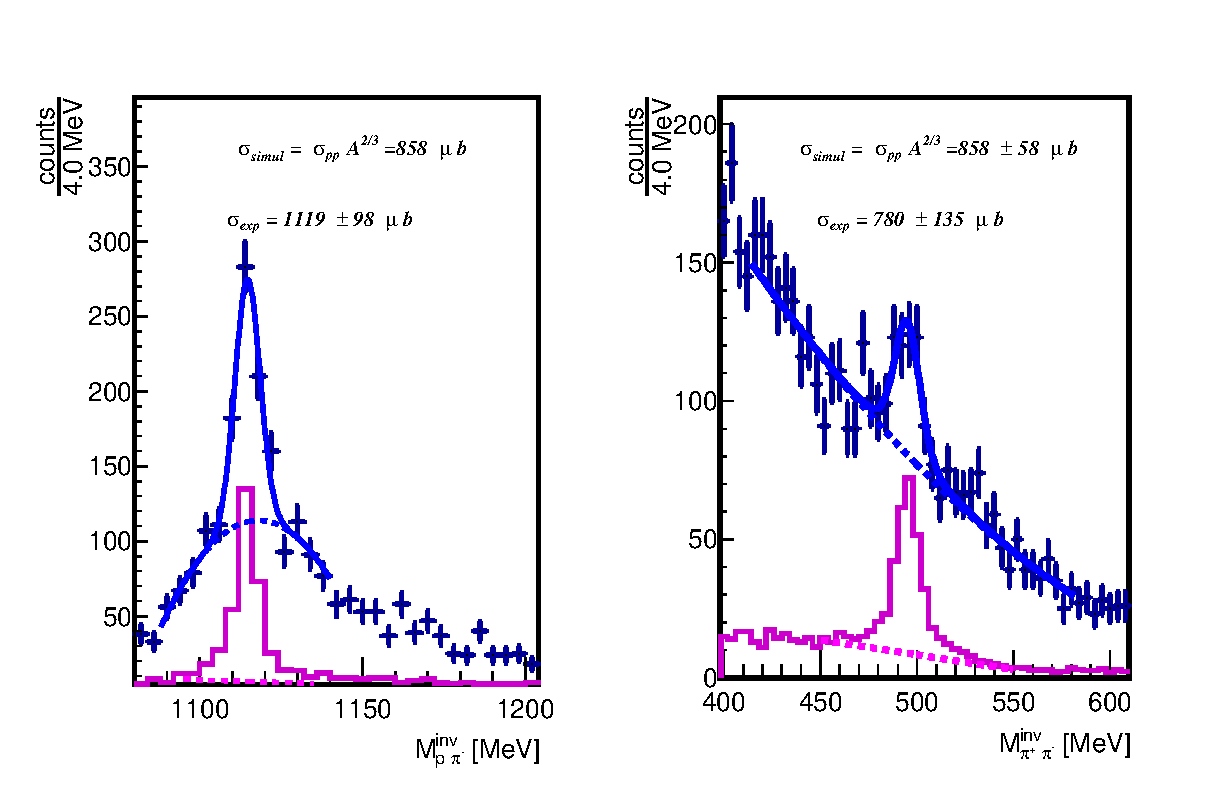
\includegraphics[width=0.9 \linewidth]{Chapter_analysisPNb/LK0.eps}
  \caption{The inclusive $\Lz \Kz$ spectrum obtained for pNb experiment. The \css for the simulation was scaled up by a factor $A^{2/3}$ compare values measured in pp reactions}
  \label{fig:LK0_pNb}
\end{figure}

\section{The $\Ls$ Reconstruction}
Compare to the $\Ls$ analysis for the pp data  for a good signal extraction a set of additional pre-cuts was necessary. They are based on cuts used for $\Lz$ reconstruction for Ag+AG collisions \cite{spies_phd}
\begin{itemize}
\item Distance between $\p \pim$ from $\Lz$
\item Distance between $\pip$ and $\pim$ from primary vertex
\item $\Lz$ vertex coordinates, reconstructed as a point of the closest approach of $\p$ and $\pim$ tracks
\item $\Ls$ vertex coordinates, reconstructed as a point of the closest approach of $\pip$ and $\pim$ tracks
\item $\Ls$ vertex coordinates, reconstructed by tracking algorithm as a primary vertex
\item Opening angle between reconstructed $\Lz$ vector and a line connecting primary and secondary vertices
\item Distance between $\p$ from $\Lz$ decay and primary vertex
\item Distance between $\pim$ from $\Lz$ decay and primary vertex
\item Distance between reconstructed $\Lz$ direction and primary vertex
\item Distance between primary and secondary vertexes
\end{itemize}




\subsection{Event mixing}


\subsection{Cross-section and extraction differential analysis}
\begin{figure}[ht]
  \centering
  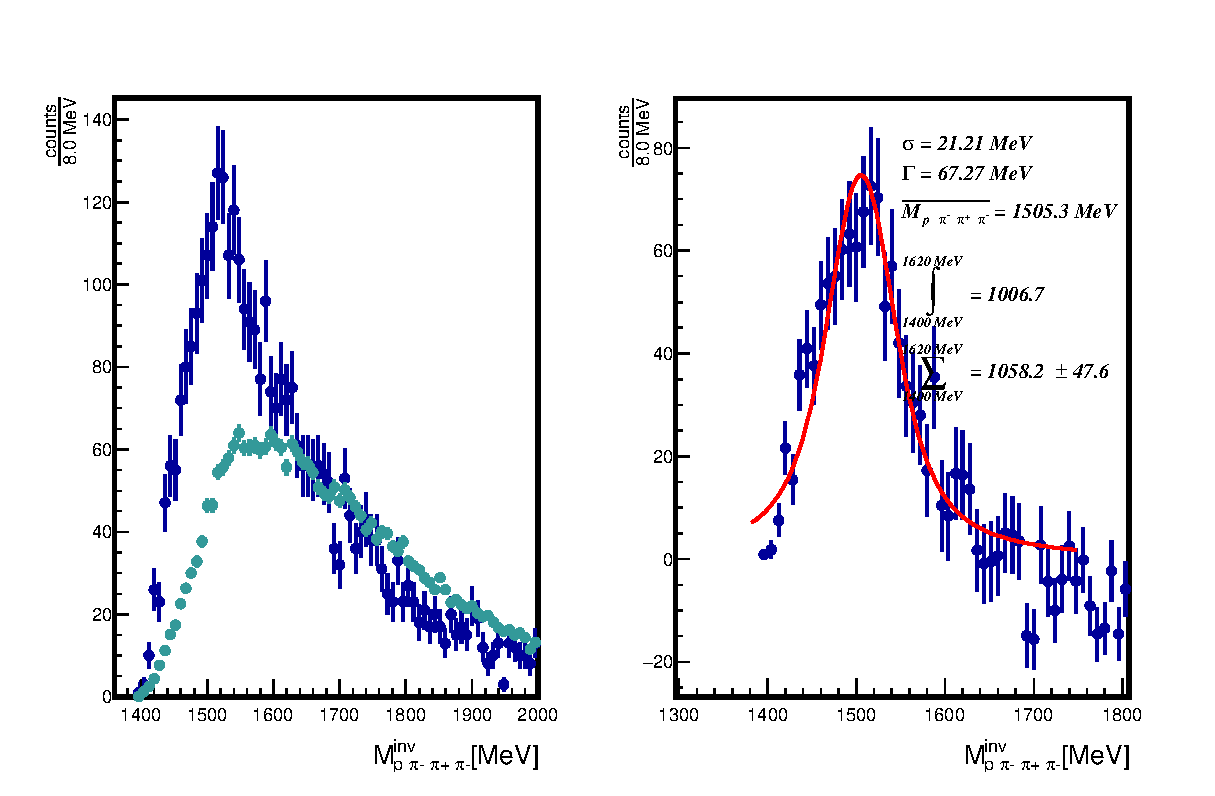
\includegraphics[width=0.9 \linewidth]{Chapter_analysisPNb/L1520.eps}
  \caption{a}
  \label{fig:L1520_pNb}
\end{figure}

\begin{figure}[ht]
  \centering
  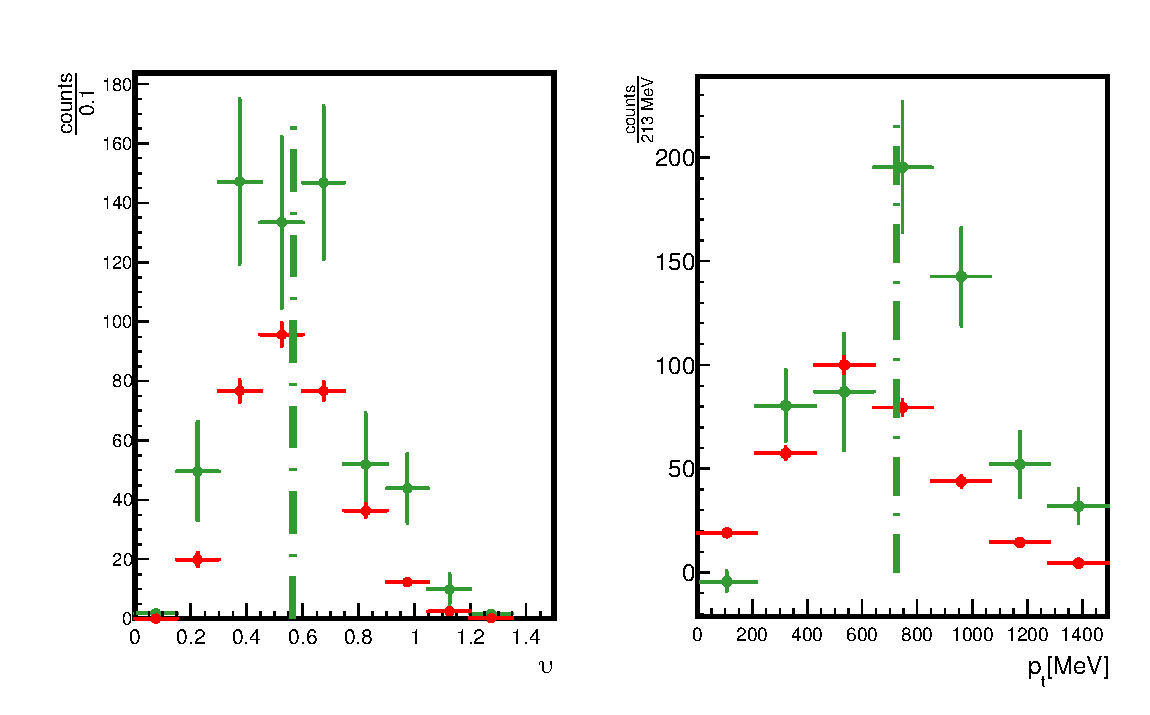
\includegraphics[width=0.9 \linewidth]{Chapter_analysisPNb/YPt.eps}
  \caption{b}
  \label{fig:YPt_pNb}
\end{figure}

\section{Comparison with results from pp data}